\documentclass[]{article}
\usepackage{lmodern}
\usepackage{amssymb,amsmath}
\usepackage{ifxetex,ifluatex}
\usepackage{fixltx2e} % provides \textsubscript
\ifnum 0\ifxetex 1\fi\ifluatex 1\fi=0 % if pdftex
  \usepackage[T1]{fontenc}
  \usepackage[utf8]{inputenc}
\else % if luatex or xelatex
  \ifxetex
    \usepackage{mathspec}
  \else
    \usepackage{fontspec}
  \fi
  \defaultfontfeatures{Ligatures=TeX,Scale=MatchLowercase}
\fi
% use upquote if available, for straight quotes in verbatim environments
\IfFileExists{upquote.sty}{\usepackage{upquote}}{}
% use microtype if available
\IfFileExists{microtype.sty}{%
\usepackage{microtype}
\UseMicrotypeSet[protrusion]{basicmath} % disable protrusion for tt fonts
}{}
\usepackage[margin=1in]{geometry}
\usepackage{hyperref}
\hypersetup{unicode=true,
            pdftitle={Global effect of temperature on phlorotannin concentration},
            pdfborder={0 0 0},
            breaklinks=true}
\urlstyle{same}  % don't use monospace font for urls
\usepackage{longtable,booktabs}
\usepackage{graphicx,grffile}
\makeatletter
\def\maxwidth{\ifdim\Gin@nat@width>\linewidth\linewidth\else\Gin@nat@width\fi}
\def\maxheight{\ifdim\Gin@nat@height>\textheight\textheight\else\Gin@nat@height\fi}
\makeatother
% Scale images if necessary, so that they will not overflow the page
% margins by default, and it is still possible to overwrite the defaults
% using explicit options in \includegraphics[width, height, ...]{}
\setkeys{Gin}{width=\maxwidth,height=\maxheight,keepaspectratio}
\IfFileExists{parskip.sty}{%
\usepackage{parskip}
}{% else
\setlength{\parindent}{0pt}
\setlength{\parskip}{6pt plus 2pt minus 1pt}
}
\setlength{\emergencystretch}{3em}  % prevent overfull lines
\providecommand{\tightlist}{%
  \setlength{\itemsep}{0pt}\setlength{\parskip}{0pt}}
\setcounter{secnumdepth}{0}
% Redefines (sub)paragraphs to behave more like sections
\ifx\paragraph\undefined\else
\let\oldparagraph\paragraph
\renewcommand{\paragraph}[1]{\oldparagraph{#1}\mbox{}}
\fi
\ifx\subparagraph\undefined\else
\let\oldsubparagraph\subparagraph
\renewcommand{\subparagraph}[1]{\oldsubparagraph{#1}\mbox{}}
\fi

%%% Use protect on footnotes to avoid problems with footnotes in titles
\let\rmarkdownfootnote\footnote%
\def\footnote{\protect\rmarkdownfootnote}

%%% Change title format to be more compact
\usepackage{titling}

% Create subtitle command for use in maketitle
\newcommand{\subtitle}[1]{
  \posttitle{
    \begin{center}\large#1\end{center}
    }
}

\setlength{\droptitle}{-2em}

  \title{Global effect of temperature on phlorotannin concentration}
    \pretitle{\vspace{\droptitle}\centering\huge}
  \posttitle{\par}
    \author{}
    \preauthor{}\postauthor{}
      \predate{\centering\large\emph}
  \postdate{\par}
    \date{08 maio, 2019}


\begin{document}
\maketitle

\subsection{Goal and hypothesis}\label{goal-and-hypothesis}

Our main goal is to understand how sea temperature affects the
production of phlorotannin by brown algae in different ocean regions
across the globe. Our general hypothesis is that temperature affects
negativelly phlorotannin concentration.

\subsection{Methods}\label{methods}

\subsubsection{Data set}\label{data-set}

We collected data from peer reviwed articles that evaluated phlorotannin
concentration produced by different species of brown algae {[}How was
the article search? Systematic search based on specific terms?{]}. We
considered each observation as the concentration of phlorotannin
produced by a particular species. From 59 references (Table S1) we
evaluated a total of 528 studies. From each study, we extracted values
of mean phlorotannin concentration, algae species and geographic
coordinates.

Based on the assumption that high temperature values restrict the
production of phlototannin bt brown algae, we represented the effect of
temperature by using maximum temperature. At each study locality we
extracted from Bio-Oracle (Tyberghein et al. 2012, Assis et al. 2017)
sea water maximum temperature at minimum depth.

\subsubsection{Statistical analysis}\label{statistical-analysis}

We used linear mixed models (LMMs) with spatial autocorrelated random
effects to examine the effects of temperature and oceanic region on
concentration of phlorotannin recorded at each site. In order to account
for spatial autocorrelated random effects we used the procedure proposed
by Rousset and Ferdy 2014 which estimates model parameters based on
Laplace approximations for the likelihood with a Matérn model (Stein
1999) for spatial correlation.

We followed the protocol of Zuur et al. (2009) to construct and test
LMMs fitted to nested and hierarchical data (i.e.replicates distributed
over species and publications). First, we built six LMMs using
combinations of random variables and selected the model with the best
random effects structure (using all fixed effects). We then used this
selected random effects structure to identify the best set of fixed
effects predictors (Table S2). In all models, the response variable was
the mean value of phlorotannin concentration (log-transformed). Ocean
region, temperature and their additive and interactive effects were
tested as fixed effect predictors. The additive effects hypothesis
assumes that both variables could influence phlorotannin concentration,
but that these effects are independent. The interactive effects
hypothesis assumes that ocean region and temperature interact to affect
phlorotannin concentration. Based on our previous random effect model
selction, species and publication identities were included in models as
random effects.

All models were compared using Akaike's information criterion (AIC),
which identifies the model that is best supported by the data (Burnham
and Anderson 2002). We also calculated Akaike evidence weights (wi). The
best-supported model was inspected and validated by residuals analysis,
which did not reveal any significant departure from model assumptions
(Figure S1). All analyses were performed using R software (R Core Team
2018), with models fitted using fitme function from spaMM package
(Rousset and Ferdy 2014). We calculated predicted values from models
using predict.HLfit from spaMM package to take into account spatial
random effects. We calculated predicted values for all temperature
values across the globe assuming spatial random effects based on a
correlation matrix between new locations and locations in the original
fit.

\subsection{Results}\label{results}

We found that phlorotannin concentration is negativelly affected by
maximum temperature. Best model retained only temperature as a fixed
effect (Table 1, Figure 1).

\begin{longtable}[]{@{}lrrrr@{}}
\caption{Table 1. Model selection results for fixed effects of
temperature (Temp), oceanic region (Ocean), and their interaction
(Temp:Ocean) based on the random effect structure: random intercept
effect of species and random intercept effect of study author. Models
were ranked based on differences in Akaike's information criterion
(AIC). k is the number of parameters in the model and w is the Akaike
weight of each model.}\tabularnewline
\toprule
Model & \(\Delta\)AIC & k & w & AIC\tabularnewline
\midrule
\endfirsthead
\toprule
Model & \(\Delta\)AIC & k & w & AIC\tabularnewline
\midrule
\endhead
Temp & 0.000000 & 2 & 0.894 & 1357.095\tabularnewline
Temp + Ocean & 4.797067 & 5 & 0.081 & 1361.892\tabularnewline
Null & 7.802578 & 1 & 0.018 & 1364.897\tabularnewline
Temp:ocean + Temp + Ocean & 10.384029 & 8 & 0.005 &
1367.479\tabularnewline
Ocean & 13.255751 & 4 & 0.001 & 1370.350\tabularnewline
\bottomrule
\end{longtable}

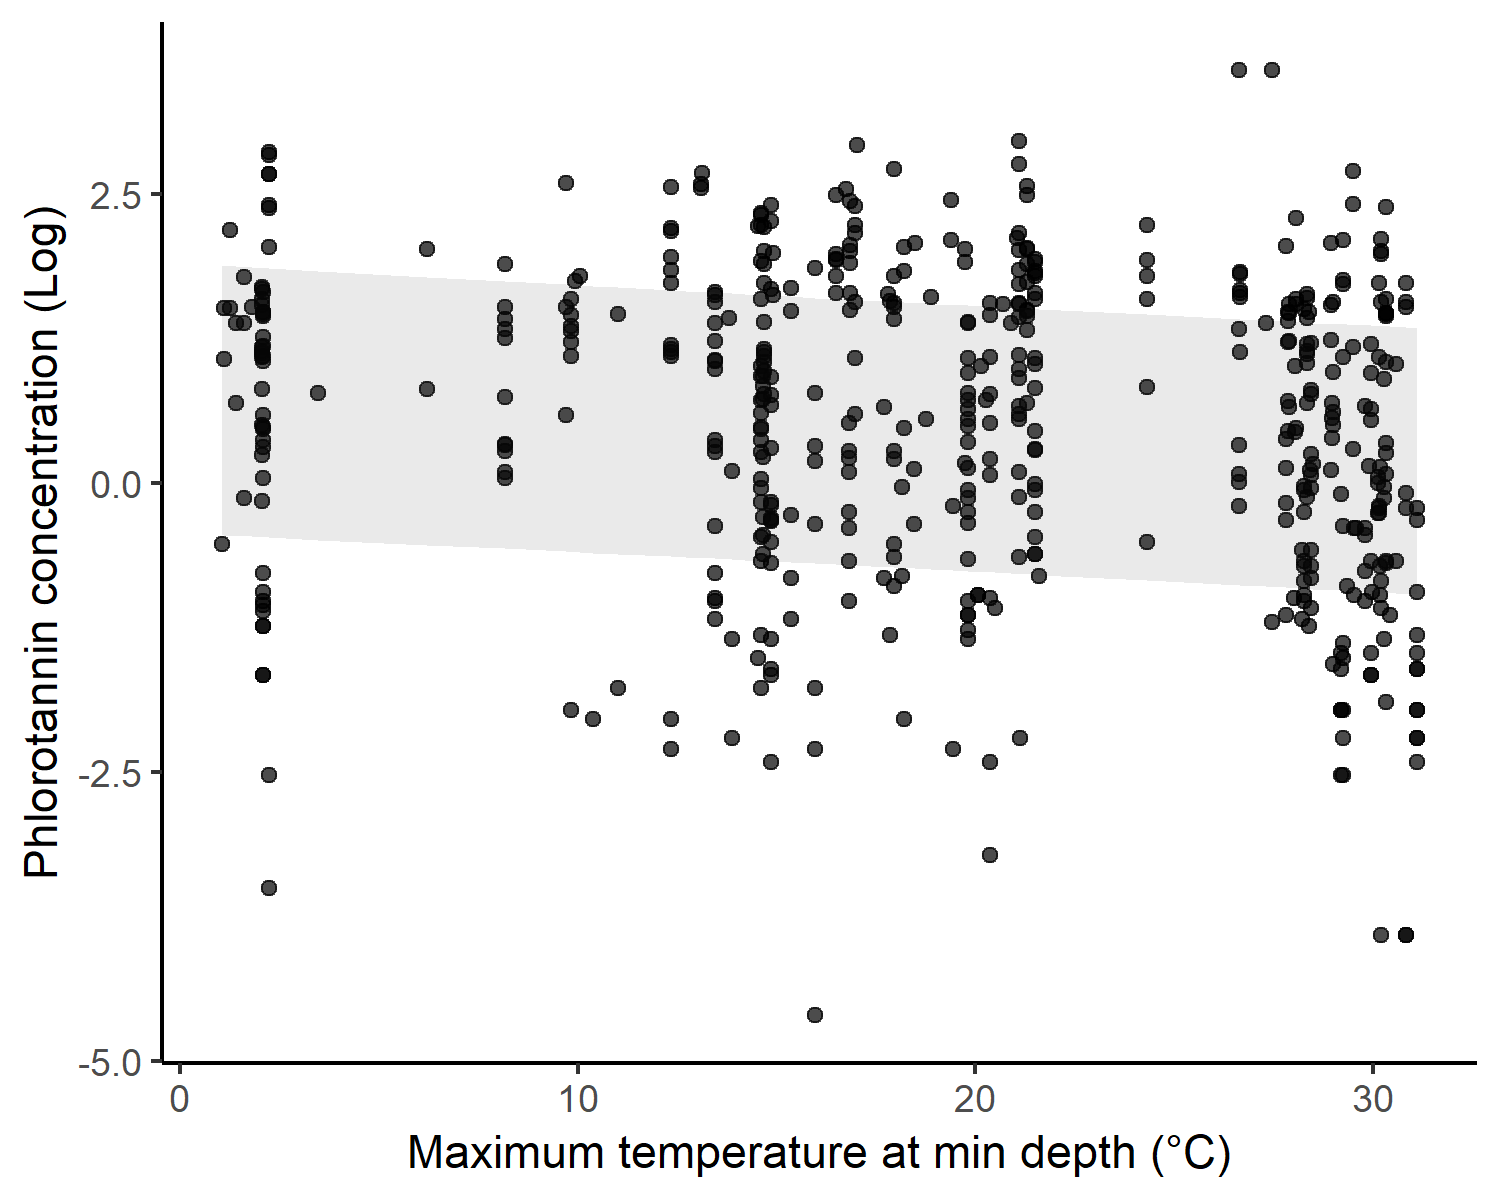
\includegraphics[width=0.60000\textwidth]{temp_vs_phlor.png}

\begin{figure}
\centering
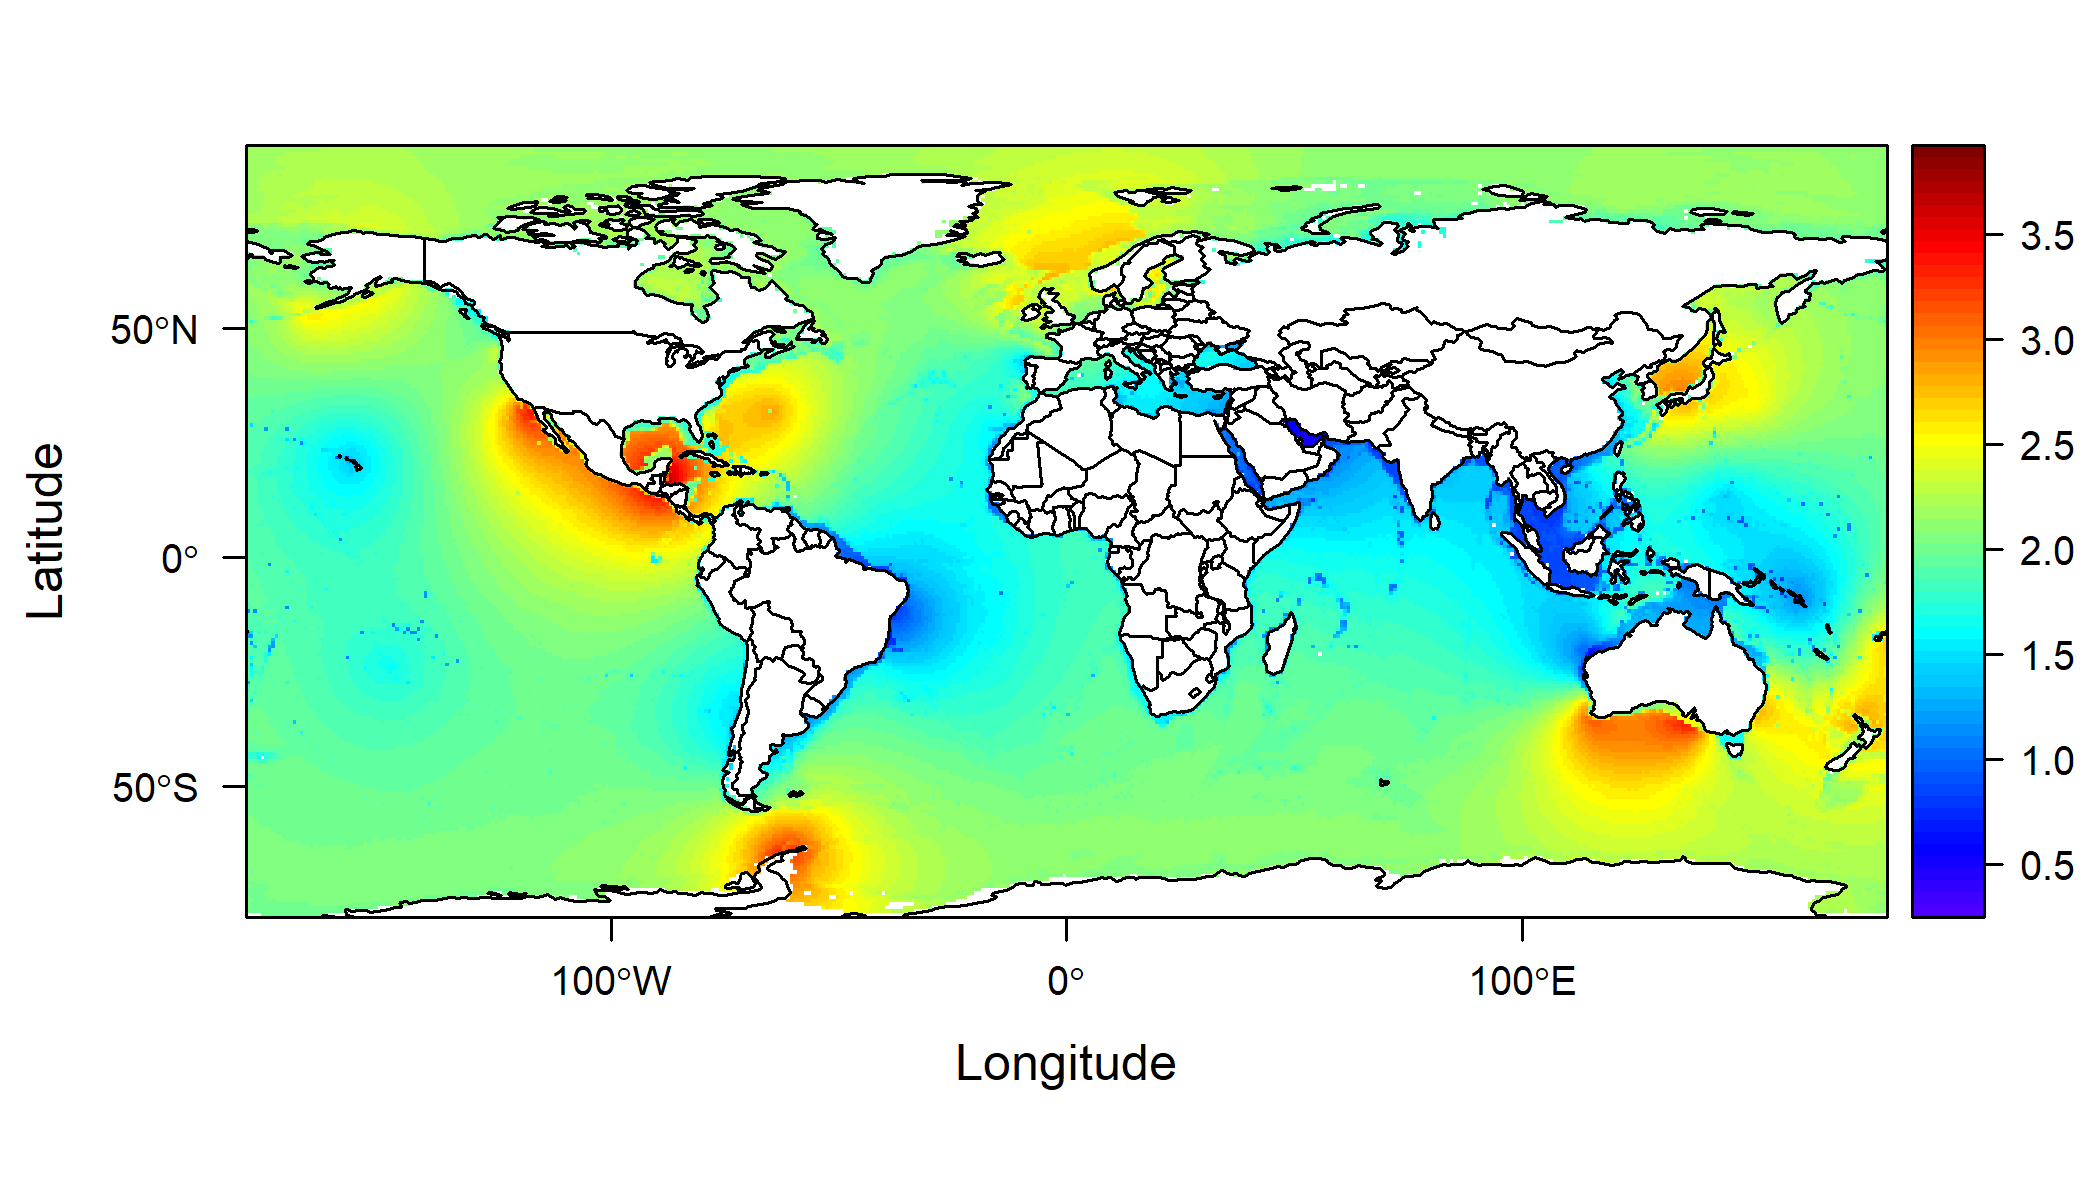
\includegraphics{predicted_map.png}
\caption{Figure 2. Prediction of phlorotannin concentration at a global
scale.}
\end{figure}


\end{document}
